\documentclass[11pt]{article}

\usepackage[a4paper]{geometry}
\geometry{left=2.0cm,right=2.0cm,top=2.5cm,bottom=2.5cm}

\usepackage{ctex} % 支持中文的LaTeX宏包
\usepackage{amsmath,amsfonts,graphicx,subfigure,amssymb,bm,amsthm,mathrsfs,mathtools,breqn} % 数学公式和符号的宏包集合
\usepackage{algorithm,algorithmicx} % 算法和伪代码的宏包
\usepackage[noend]{algpseudocode} % 算法和伪代码的宏包
\usepackage{fancyhdr} % 自定义页眉页脚的宏包
\usepackage[framemethod=TikZ]{mdframed} % 创建带边框的框架的宏包
\usepackage{fontspec} % 字体设置的宏包
\usepackage{adjustbox} % 调整盒子大小的宏包
\usepackage{fontsize} % 设置字体大小的宏包
\usepackage{tikz,xcolor} % 绘制图形和使用颜色的宏包
\usepackage{multicol} % 多栏排版的宏包
\usepackage{multirow} % 表格中合并单元格的宏包
\usepackage{pdfpages} % 插入PDF文件的宏包
\RequirePackage{listings} % 在文档中插入源代码的宏包
\RequirePackage{xcolor} % 定义和使用颜色的宏包
\usepackage{wrapfig} % 文字绕排图片的宏包
\usepackage{bigstrut,multirow,rotating} % 支持在表格中使用特殊命令的宏包
\usepackage{booktabs} % 创建美观的表格的宏包
\usepackage{circuitikz} % 绘制电路图的宏包
\usepackage{caption}
\captionsetup{font=normalsize,skip=2pt}

\definecolor{dkgreen}{rgb}{0,0.6,0}
\definecolor{gray}{rgb}{0.5,0.5,0.5}
\definecolor{mauve}{rgb}{0.58,0,0.82}
\lstset{
  frame=tb,
  aboveskip=3mm,
  belowskip=3mm,
  showstringspaces=false,
  columns=flexible,
  framerule=1pt,
  rulecolor=\color{gray!35},
  backgroundcolor=\color{gray!5},
  basicstyle={\small\ttfamily},
  numbers=none,
  numberstyle=\tiny\color{gray},
  keywordstyle=\color{blue},
  commentstyle=\color{dkgreen},
  stringstyle=\color{mauve},
  breaklines=true,
  breakatwhitespace=true,
  tabsize=3,
}

% 轻松引用, 可以用\cref{}指令直接引用, 自动加前缀. 
% 例: 图片label为fig:1
% \cref{fig:1} => Figure.1
% \ref{fig:1}  => 1
\usepackage[capitalize]{cleveref}
% \crefname{section}{Sec.}{Secs.}
\Crefname{section}{Section}{Sections}
\Crefname{table}{Table}{Tables}
\crefname{table}{Table.}{Tabs.}

\setmainfont{Palatino_Linotype}[
  Path = ../Fonts/,
  Extension = .ttf
]
\setCJKmainfont{SimHei}[
  Path = ../Fonts/,
  Extension = .ttf
]
\punctstyle{kaiming}
% 偏好的几个字体, 可以根据需要自行加入字体ttf文件并调用

\renewcommand{\emph}[1]{\begin{kaishu}#1\end{kaishu}}

%改这里可以修改实验报告表头的信息
\newcommand{\studentNum}{00000000}
\newcommand{\name}{我是谁}
\newcommand{\exDate}{2025.04.15}
\newcommand{\weekDay}{二}
\newcommand{\ap}{下午}
%%%%%%%%%%%%%%%%%%%%%%%%%%%

\begin{document}

%若需在页眉部分加入内容, 可以在这里输入
% \pagestyle{fancy}
% \lhead{\kaishu 测试}
% \chead{}
% \rhead{}

\begin{center}
    \LARGE \bf 《\, 基\, 础\, 物\, 理\, 实\, 验\, 》\, 实\, 验\, 报\, 告
\end{center}

\begin{center}
    \emph{学号}\underline{\makebox[6em][c]{\studentNum}}
    \emph{姓名}\underline{\makebox[6em][c]{\name}} 
    \emph{实验日期} \underline{\makebox[8em][c]{\exDate}}
    \emph{星期} \underline{\makebox[2em][c]{\weekDay}}\;\underline{\makebox[3em][c]{\ap}}
    {\noindent}
    \rule[8pt]{17cm}{0.2em}
\end{center}

\begin{center}
    \Large \bf 半导体热敏电阻特性的研究(平衡电桥)
\end{center}

\section*{一、实验目的}

\begin{enumerate}
    \item 了解热敏电阻的电阻-温度特性和测温原理
    \item 掌握惠斯通电桥的原理和使用方法
\end{enumerate}

\section*{二、实验原理}


1. 半导体热敏电阻的电阻-温度特性
    
半导体热敏电阻的基本特性是它的温度特性,而这种特性又是与半导体材料的导电机制密切相关的。由于半导体中的载流子数目随温度升高而按指数规律迅速增加。温度越高,载流子的数目越多,导电能力越强,电阻率也就越小。因此热敏电阻随着温度的升高,它的电阻将按指数规律迅速减小。

实验表明,在一定温度范围内,半导体材料的电阻$R_T$和绝对温度$T$的关系可表示为
\begin{align}
    R_T=ae^{\frac{b}{T}}
\end{align}
其中常数$a$不仅与半导体材料的性质而且与它的尺寸均有关系,而常数$b$仅与材料的性质有关,$T$取绝对温度。

定义电阻温度系数为:
\begin{align}
    \alpha=\dfrac{1}{R_T}\dfrac{dR_T}{dT}
\end{align}

按照温度系数不同分为和负温度系数,正温度系数热敏电阻在温度越高时电阻值越大,负温度系数热敏电阻在温度越高时电阻值越低。

$(1)$式中常数$a$、$b$可通过实验方法测得。常利用多个$T$和$R_T$的组合测量值,通过作图的方法(或用回归法最好)来确定常数$a$、$b$,为此取$(1)$式两边的对数。变换成直线方程:
\begin{align}
    \ln R_T=\ln a+\dfrac{b}{T}
\end{align}
或写作$Y=A+BX$的形式,其中$Y=\ln R_T$,$A=\ln a$,$B=b$,$X=\dfrac{1}{T}$。,然后取$X$、$Y$分别为横、纵坐标,对不同的温度$T$测得对应的$R_T$值,经过变换后作$X-Y$曲线,它应当是一条截距为$A$、斜率为$B$的直线。根据斜率求出$b$,又由截距可求出$a=e^A$。

确定了半导体材料的常数$a$和$b$后,便可计算出这种材料的电阻温度系数
\begin{align}
    \alpha=\dfrac{1}{R_T}\dfrac{dR_T}{dT}=-\dfrac{b}{T^2}\times100\%
\end{align}

\begin{wrapfigure}{r}{4cm}
    \centering
    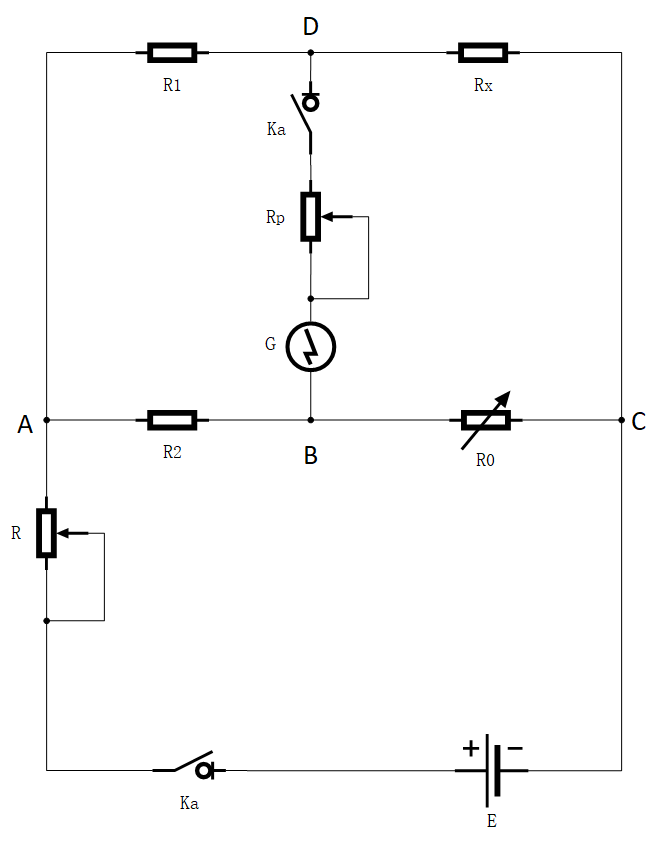
\includegraphics[width=4cm]{Figs/实验原理图.png}
    \caption{\small 实验原理图}
\end{wrapfigure}

显然,半导体热敏电阻的温度系数是负的,并与温度有关。

2. 用惠斯顿电桥测量半导体热敏电阻

惠斯顿电桥的原理图如图$1$所示, 四个电阻$R_0$,$R_1$,$R_2$,$R_x$组成一个四边形,即电桥的四个臂,其中$R_x$就是待测电阻。在四边形的一对对角$A$和$C$之间连接电源,而在另一对对角$B$和$D$之间接入检流计$G$。当$B$和$D$两点电位相等时,$G$中无电流通过,电桥便达到了平衡。平衡时必有
\begin{align}
    R_x=\dfrac{R_1}{R_2}R_0
\end{align}

$R_1$、$R_2$和$R_0$都已知,$R_x$即可求出。

\section*{三、实验仪器}

箱式惠斯通电桥、控温仪、热敏电阻、直流电稳压电源。

\section*{四、实验内容}

\begin{enumerate}
    \item 求电桥灵敏度
    
    本实验中为测量电桥灵敏度,可以先调电桥至平衡,$R_x=R_0=3000\Omega$,$\dfrac{R_1}{R_2}=1$,改变$R_x$至$R_x+\Delta R_x$,使检流计偏转$15$格;再将$R_x$改变为$R_x-\Delta R_x$,使检流计向反方向偏转$15$格,取两次$\Delta R_x$的平均值$\overline{\Delta R_x}$,带入公式$s=\dfrac{\Delta n}{\dfrac{\overline{\Delta R_x}}{R_x}}$得到电桥灵敏度。
    \item 测量热敏电阻的温度特性
    
    接好电路,安置好仪器。

    将热敏电阻放入加热铜管,温度由自动温控仪控制。热敏电阻的两条引出线连接到惠斯通电桥的待测电阻$R_x$的接线柱上。

    测试的温度从$30^{\circ}C$开始,每增加$2.5^{\circ}C$,测量温度点的$R_t$,直到$70^{\circ}C$止。绘制热敏电阻$R_T-T$特性曲线。由电阻的温度系数定义式,在$T=50^{\circ}C$的点作切线,求出该点切线的斜率、$T=50^{\circ}C$点的电阻温度系数。

    作$\ln R_T-\dfrac{1}{T}$曲线,确定式$(1)$中常数$a$和$b$,再由$(4)$式求$T=50^{\circ}C$时的电阻温度系数$\alpha\;(\alpha=-\dfrac{b}{T^2})$,并将两次求得的$\alpha$进行对比。
\end{enumerate}

\section*{五、数据记录}

原始数据见附录。

\section*{六、数据处理}

1. 求电桥灵敏度

\begin{align*}
    \overline{\Delta R_x}&=\dfrac{\Delta R_{x_1}+\Delta R_{x_2}}{2}=\dfrac{23.7+23.3}{2}\Omega=22.5\Omega \\
    s&=\dfrac{\Delta n}{\dfrac{\overline{\Delta R_x}}{R_x}}=\dfrac{15}{\dfrac{22.5\Omega}{3000\Omega}}=2000
\end{align*}

2. 热敏电阻温度特性

将摄氏温标转换为开氏温标,对正向与反向的电阻取平均值,见图$2$。
\begin{figure}[H]
    \centering
    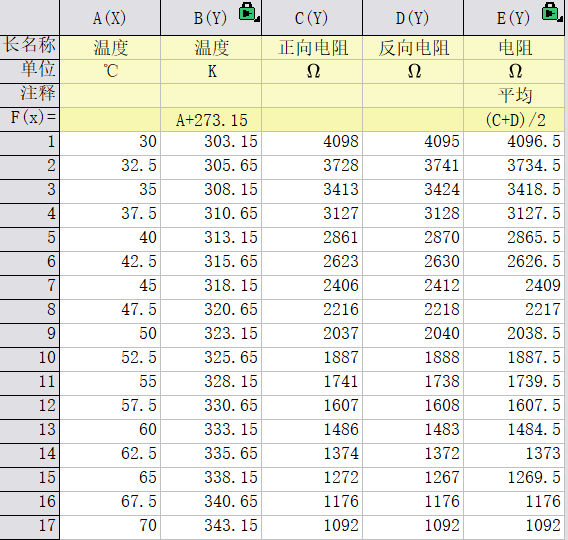
\includegraphics[width=10cm]{Figs/数据.png}
    \caption{数据表}
\end{figure}

绘制热敏电阻$R_T-T$散点图,并用$y=Ae^{\frac{B}{x}}$作拟合曲线,然后再$50^{\circ}C$处作切线,如图$3$所示。
\begin{figure}[H]
    \centering
    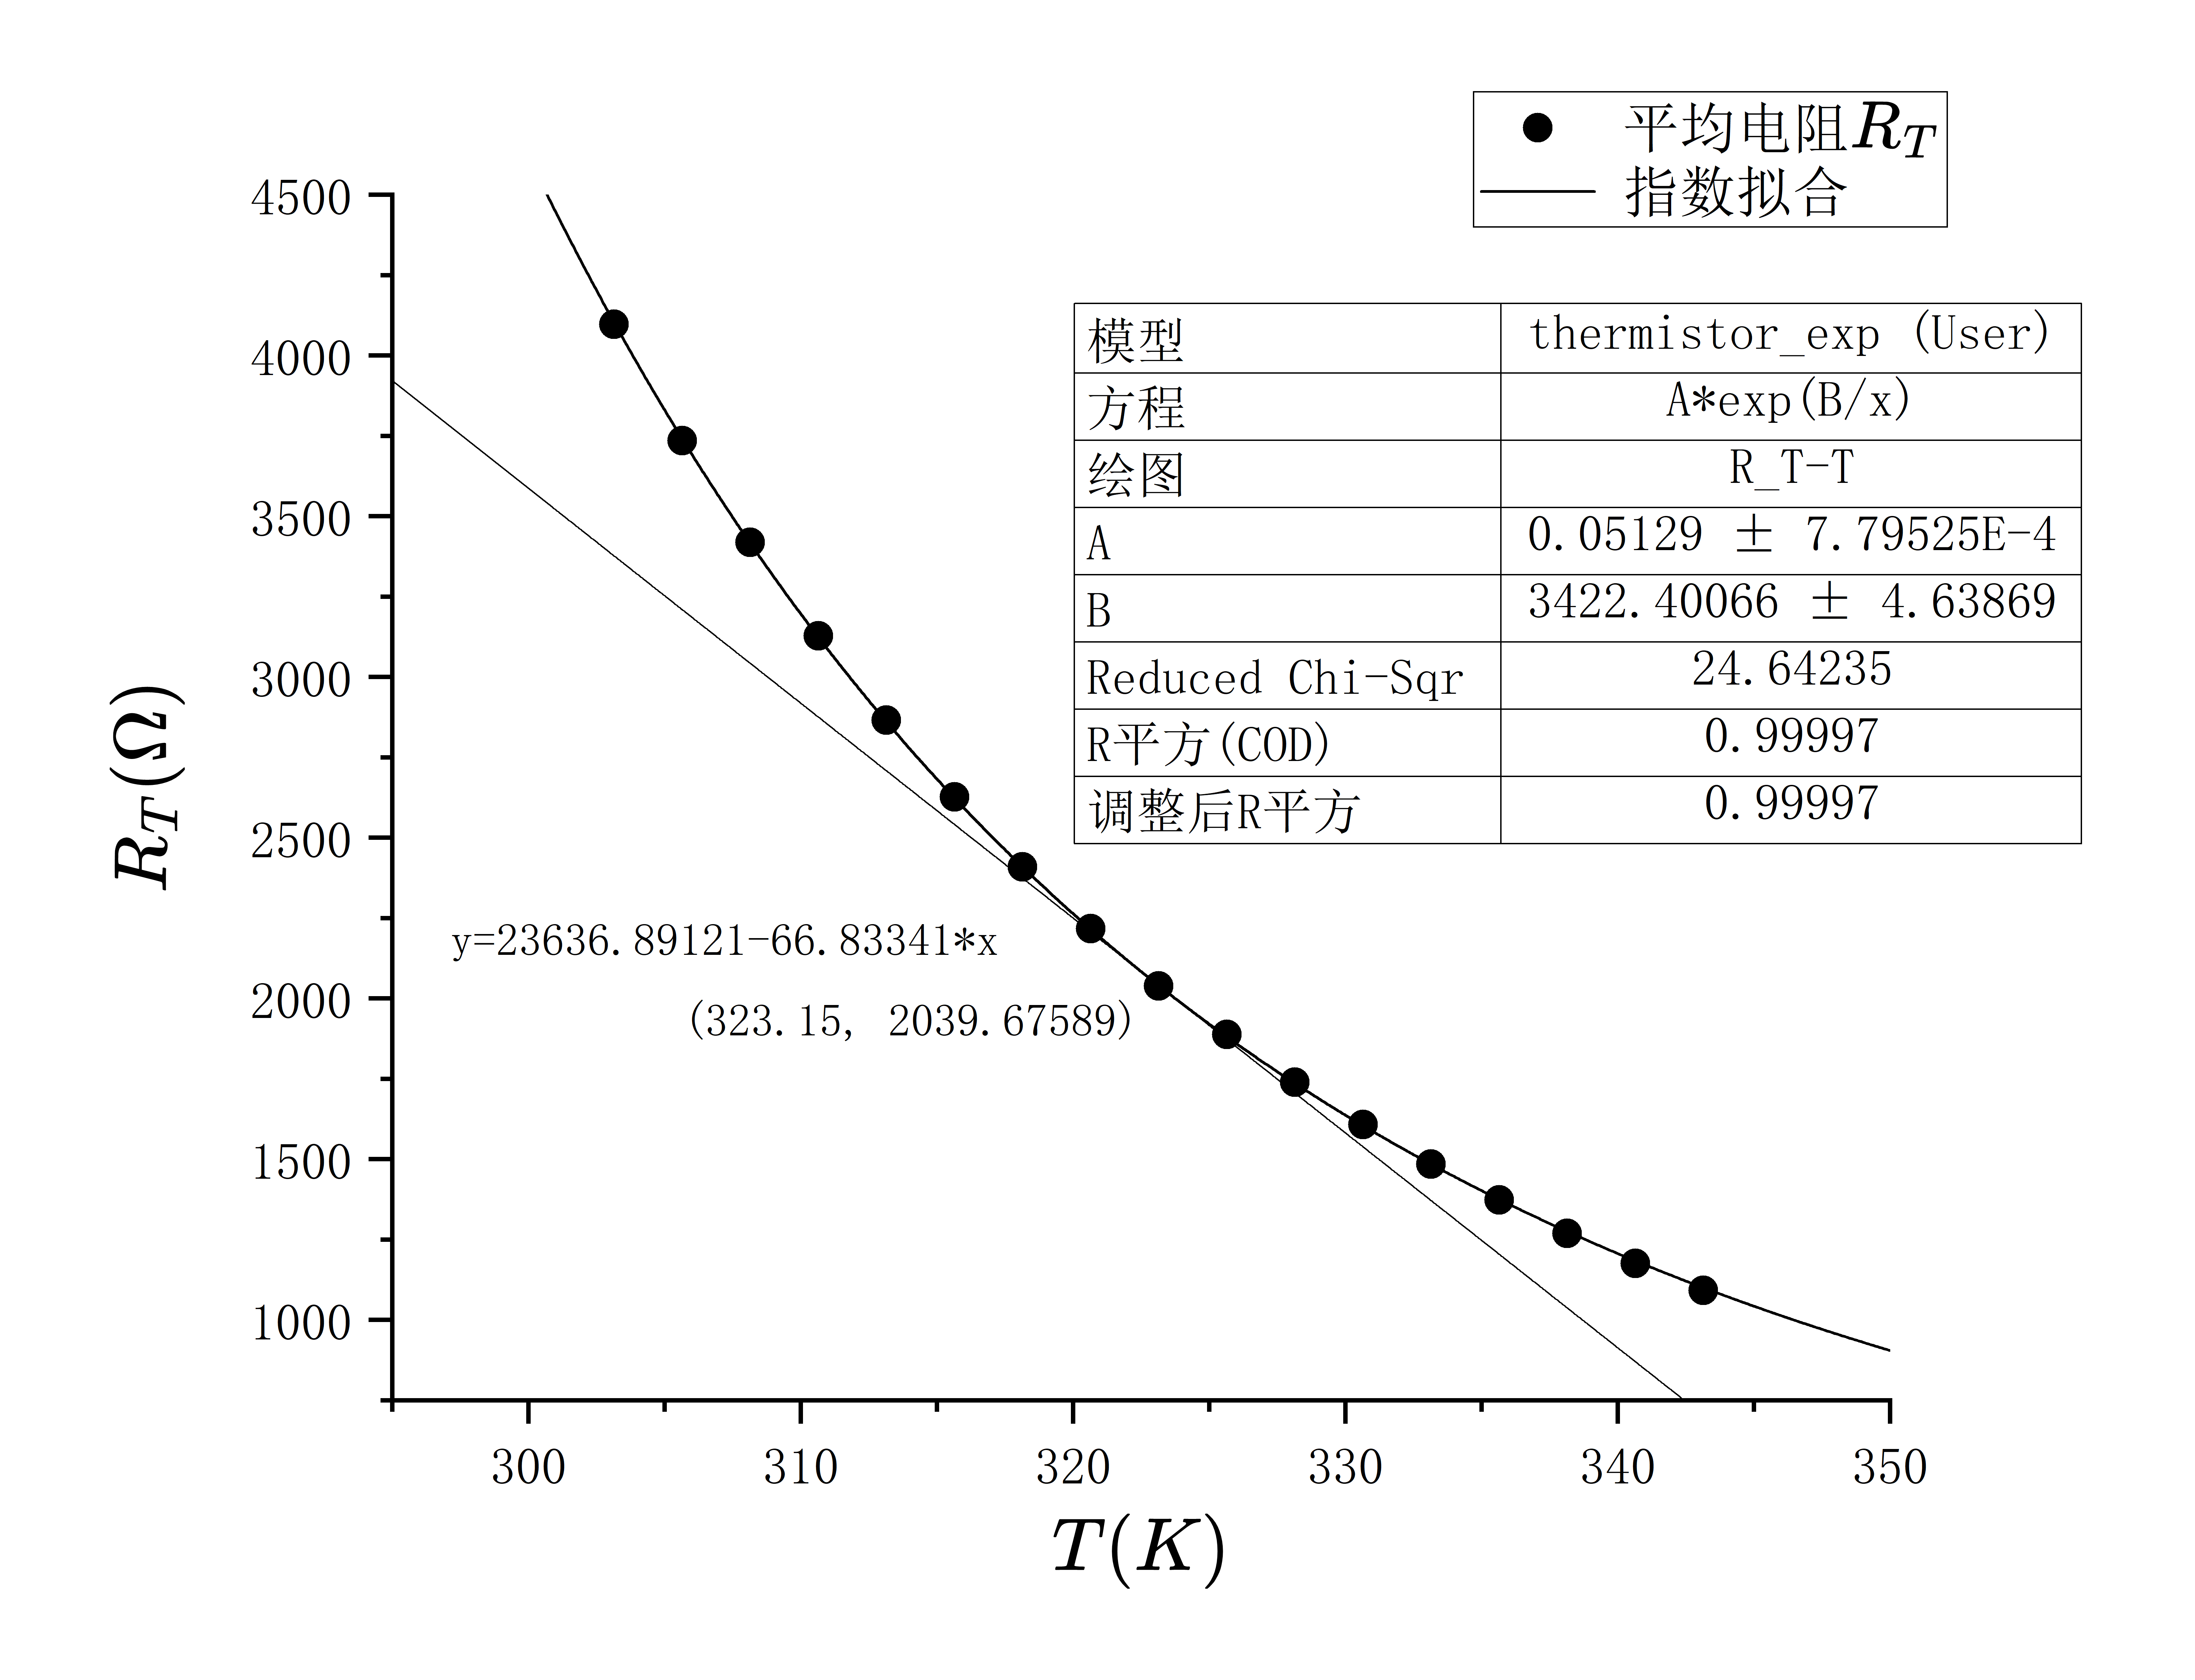
\includegraphics[width=16cm]{Figs/Graph1.png}
    \caption{热敏电阻$R_T-T$特性曲线及其指数拟合与$T=50^{\circ}C$处的切线}
\end{figure}
得到拟合曲线方程为$y=0.05129e^{\frac{3422.40066}{x}}$,$T=50^{\circ}C$处的切线方程为$y=-66.83341x+23636.89121$,故斜率为$-66.83341$。通过带入$(2)$式可得到电阻温度系数为$\alpha_1=\dfrac{-66.83341}{2038.5}=-0.03279\;/^{\circ}C$

将$R_T$取对数,$T$取倒数,作$\ln(R_T)-\dfrac{1}{T}$散点图以及线性拟合曲线,如图$4$所示。
\begin{figure}[H]
    \centering
    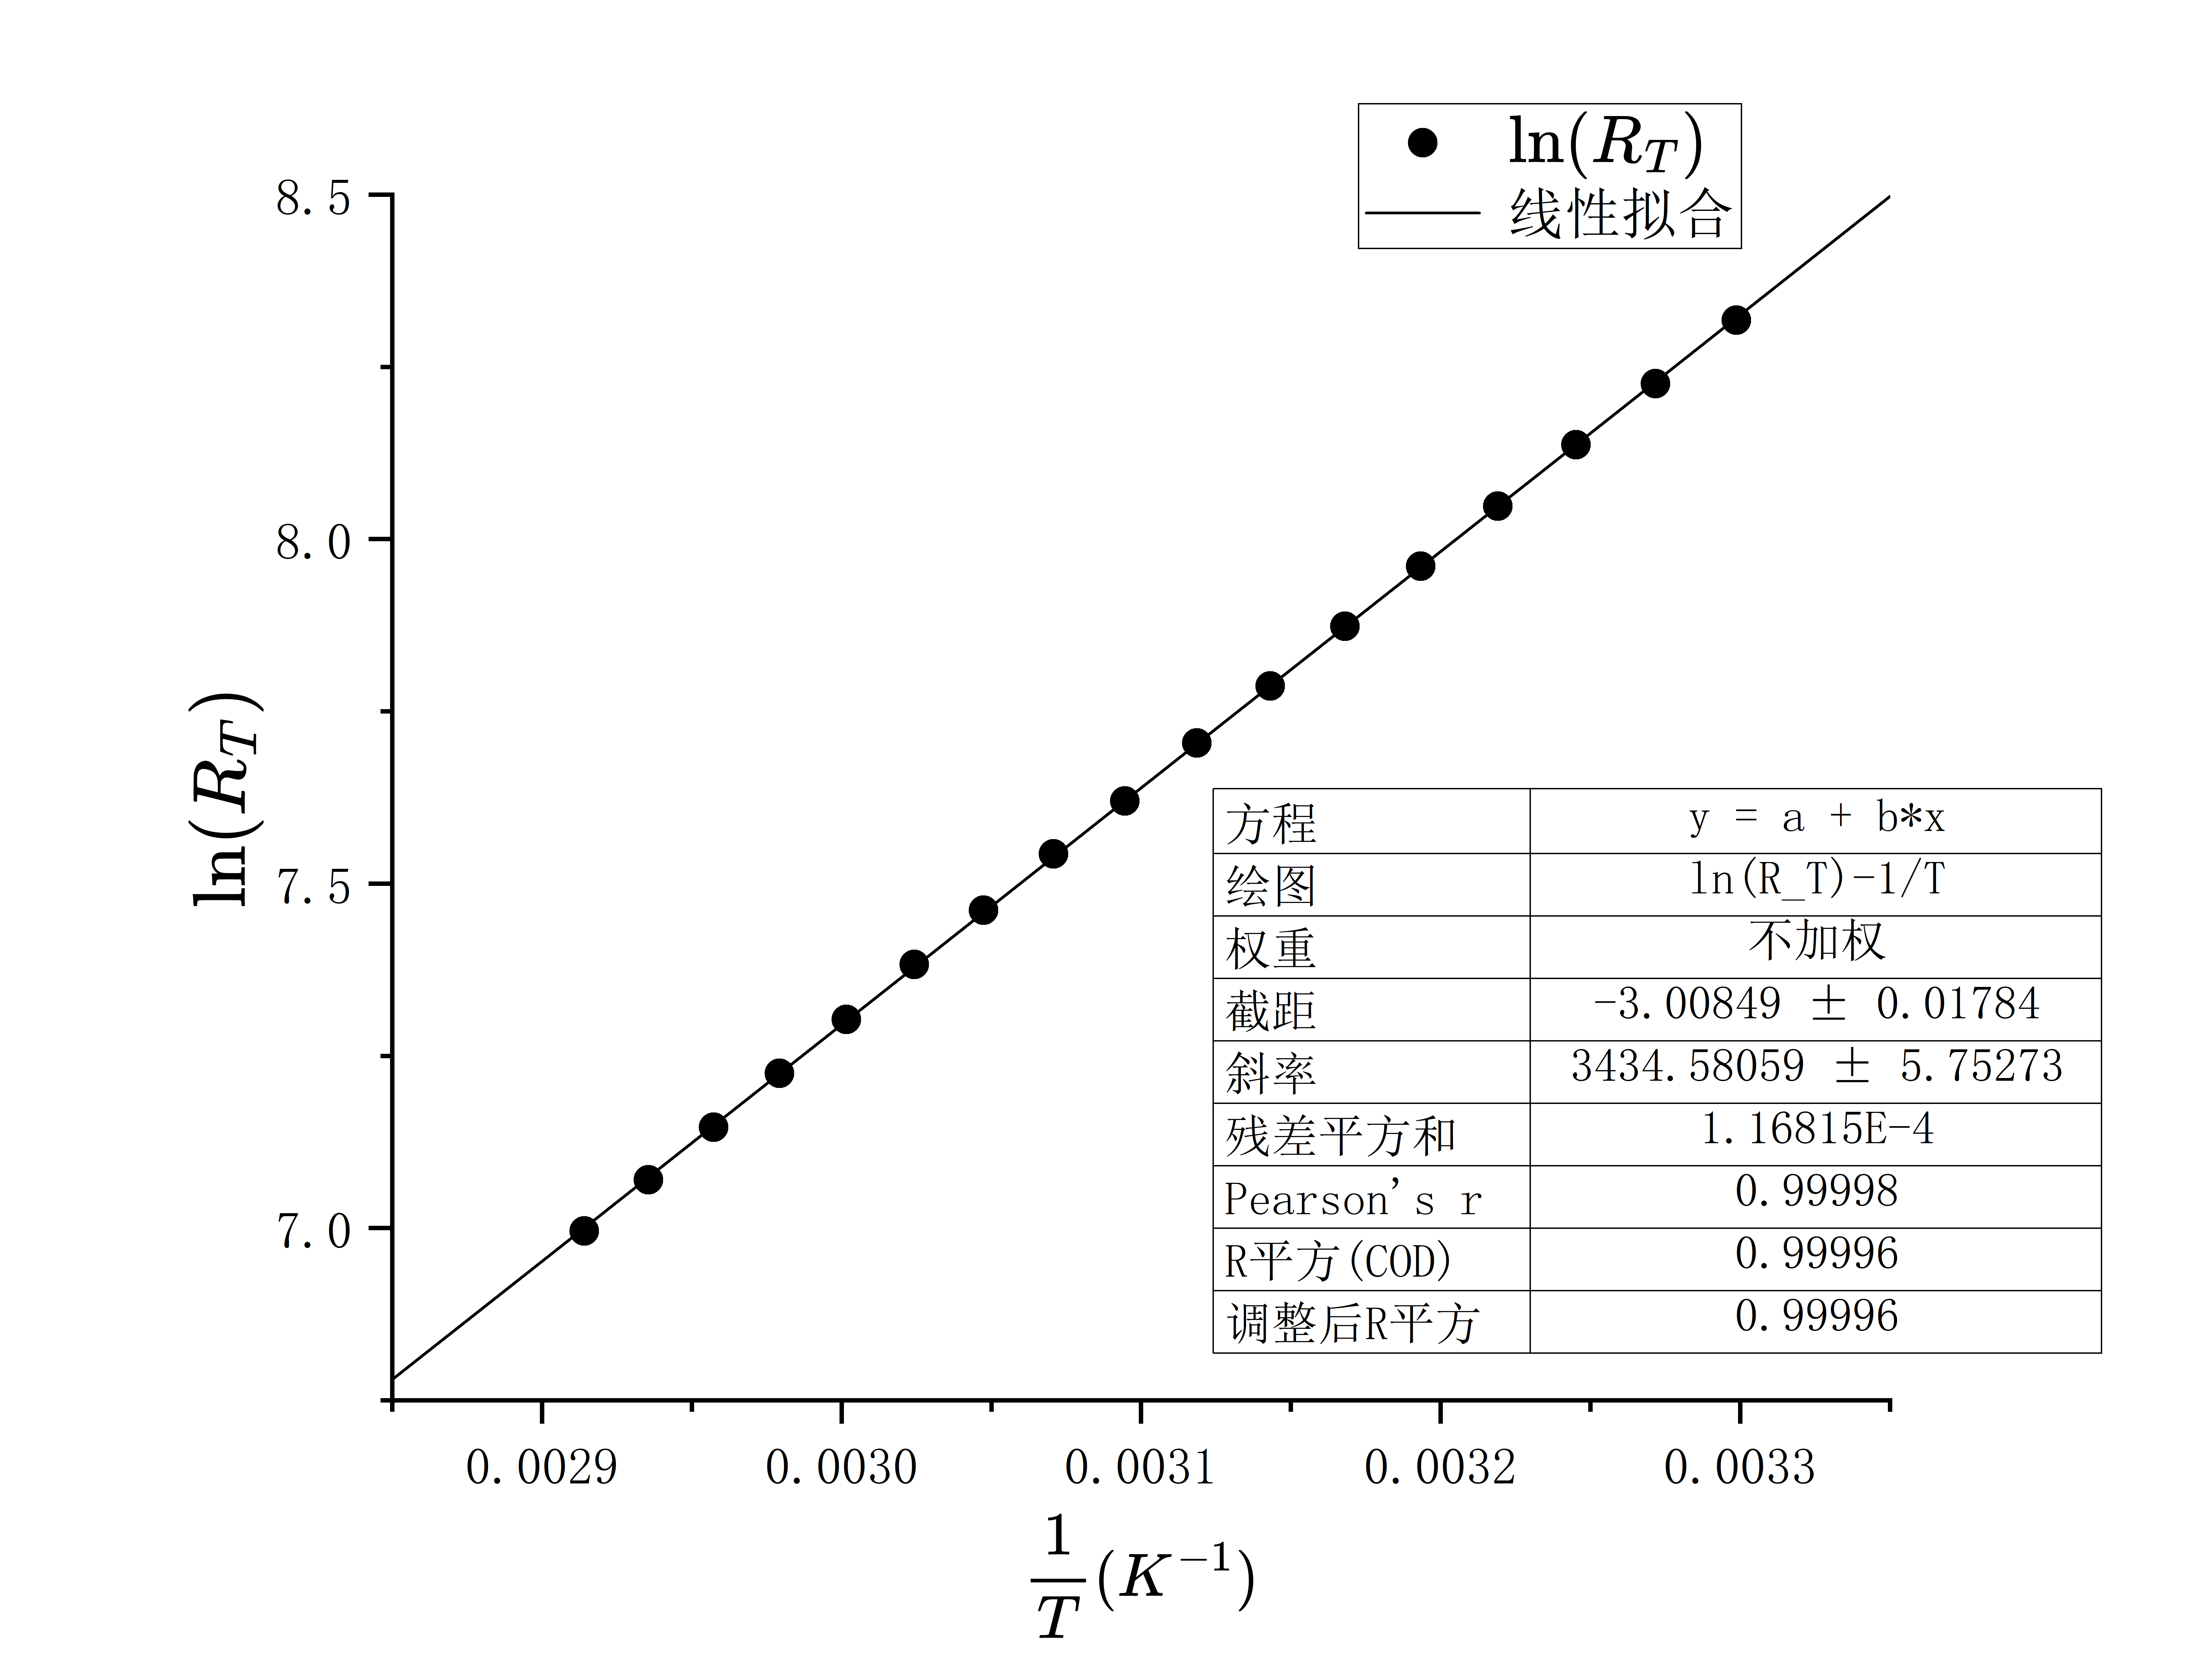
\includegraphics[width=16cm]{Figs/Graph2.png}
    \caption{热敏电阻$\ln(R_T)-\dfrac{1}{T}$特性曲线及其线性拟合}
\end{figure}
得到拟合直线方程为$y=3434.58059x-3.00849$。根据$(4)$式可知得到$\alpha_2=-\dfrac{k}{T^2}=-\dfrac{3434.58059}{323.15^2}=-0.03289\;/^{\circ}C$

对比$\alpha_1$与$\alpha_2$
$$\left|\dfrac{\alpha_2-\alpha_1}{\alpha1}\right|=\left|\dfrac{-0.03289+0.03279}{-0.03279}\right|=3.049\times10^{-3}=0.3049\%
$$
$$\left|\dfrac{\alpha_1-\alpha_2}{\alpha2}\right|=\left|\dfrac{-0.03279+0.03289}{-0.03289}\right|=3.040\times10^{-3}=0.3040\%
$$
故可以得出$\alpha_1\approx\alpha_2$,故该热敏电阻在$50^{\circ}C$时的电阻温度系数为
$$
\alpha=\dfrac{\alpha_1+\alpha_2}{2}=\dfrac{-0.03279-0.03289}{2}=-0.03284\;/^{\circ}C=-3.284\%/^{\circ}C
$$

\section*{七、误差分析}

\begin{enumerate}
    \item 自动温控仪控温会在$0.1^{\circ}C$内波动,使得电阻读数不准;
    \item 电桥的电阻调节最小刻度为$1\Omega$,不够精确;
    \item 开关与导线本身有电阻,使得结果不准确;
    \item 使用时间久导致电桥电阻会发热而阻值不准确。
\end{enumerate}

\section*{八、思考题}

\begin{enumerate}
    \item 在多次测量灵敏度的时候,试分析每次需要重测初始电阻吗?
    
    答:本实验中的$R_0, R_x$为固定值$3000\Omega$,比例臂$\dfrac{R_1}{R_2}$固定为$1:1$,故无需重新测量,重新测量反而会带来更多的系统误差。但若按照正常流程,即通过调节$R_0$测量计算初始电阻$R_x$,并且改变$R_0$来使检流记偏转,需要重新测量初始电阻,因为电阻或电桥内部元件受温度影响,阻值可能发生微小漂移;电桥开关或接线端子接触不良会导致初始平衡条件改变;电源电压波动可能影响电桥平衡点。导致初始电阻未校准,后续测量的$\Delta R_x$和灵敏度$s$将偏离真实值,导致结果不可靠。
    \item 测量热敏电阻的阻值,如果没有等温度稳定就记录实验结果,试分析对结果的影响?
    
    答:会导致误差。热敏电阻的阻值随温度动态变化。若温度未稳定时记录数据,测得的$R_T$对应的是瞬时温度下的而非设定温度下的,导致$R_T-T$曲线偏离真实特性。若温度波动剧烈,数据点会分散,降低拟合精度。若每个点测量温度都比设定温度略低,则导致测得$R_T$偏高,使得对数法拟合得到的斜率偏大而使温度系数的绝对值偏大,温度未稳定会导致切线斜率不准确,进一步影响$\alpha$的计算。
\end{enumerate}

\section*{九、实验结论}

实验所用的惠斯特电桥灵敏度为$s=2000$,此热敏电阻在$50^{\circ}C$时的电阻温度系数为$\alpha=-0.03284\;/^{\circ}C=-3.284\%/^{\circ}C$

\end{document}